\documentclass[conference]{IEEEtran}
\IEEEoverridecommandlockouts
% The preceding line is only needed to identify funding in the first footnote. If that is unneeded, please comment it out.
\usepackage{cite}
\usepackage{amsmath,amssymb,amsfonts}
\usepackage{algorithmic}
\usepackage{graphicx}
\usepackage{hyperref}
\usepackage{textcomp}
\usepackage{xcolor}
\def\BibTeX{{\rm B\kern-.05em{\sc i\kern-.025em b}\kern-.08em
    T\kern-.1667em\lower.7ex\hbox{E}\kern-.125emX}}
\begin{document}

\title{High-speed SWIR Hyperspectral Imaging For Material Classification In Operating Room\\
% {
% \footnotesize 
% \textsuperscript{*}Note: Sub-titles are not captured in Xplore and should not be used}
% \thanks{Identify applicable funding agency here. If none, delete this.}
}

% \author{

% \IEEEauthorblockN{Yunan Wang}
% \IEEEauthorblockA{
% % \textit{} \\
% \textit{Rice University}\\
% Houston, TX \\
% yw256@rice.edu}
% \and}

\author{
\IEEEauthorblockN{Yunan Wang, Lauren Gold, Kevin F. Kelly，Robert LiKamWa}
\IEEEauthorblockA{Department of Electrical and Computer Engineering\\
Rice University, Houston, TX 77005 USA}}

% <-this % stops an unwanted space


\maketitle
\begin{abstract}
Intraoperative tissue classification requires fast and reliable imaging tools for real-time surgical guidance. Although hyperspectral imaging provides rich spectral information, most existing systems rely on spectral or spatial scanning and are too slow for clinical use. To address this limitation, we present a high-speed short-wave-infrared (SWIR) hyperspectral projector based on structured illumination and compressive sensing. Spectral information is encoded at the illumination stage using a digital micromirror device, and the resulting measurements are decoded to recover spectral features for tissue classification. By shifting spectral multiplexing to the projection stage, the proposed framework enables faster acquisition and provides a foundation for real-time SWIR hyperspectral imaging.
\end{abstract}

\begin{IEEEkeywords}
SWIR, Hyperspectral Imaging, Material Classification, Compressive Sensing, Computer Vision.
\end{IEEEkeywords}

\section{Introduction}
Intraoperative tissue assessment plays a critical role in many surgical procedures, where fast and reliable imaging tools are required to support real-time clinical decision-making. For example, accurate evaluation of burn severity\cite{2020Burn}, cutaneous inflammation\cite{Du2020SWIRDermatitis}, or identification of diseased tissue margins directly influences surgical outcomes and treatment planning. Conventional visual inspection is often subjective and may fail to capture subtle physiological differences across tissue types. These limitations motivate the development of quantitative optical imaging techniques capable of providing rapid, non-contact, and information-rich measurements during surgery.

Hyperspectral imaging (HSI) has emerged as a promising modality for biomedical applications \cite{Bhargava2024HSIReview,Golovynskyi2023Lipids} due to its ability to capture detailed spectral signatures associated with tissue composition. In particular, imaging in the short-wave infrared (SWIR) spectral range offers several advantages over visible and near-infrared regimes. Reduced scattering in biological tissue enables improved penetration depth and more stable reflectance measurements, while stronger absorption features related to water and lipid content provide enhanced sensitivity to physiological variations\cite{Wilson2015SWIRReview, Roblyer2025SWIRReview, Wilson2025SWIRDecade}. These properties make SWIR hyperspectral imaging attractive for intraoperative tissue classification tasks.

Despite its potential, the clinical translation of hyperspectral imaging remains limited by acquisition speed. Most existing HSI systems rely on spectral or spatial scanning mechanisms\cite{Gao2010IMS,Antony2024HSIReview,Stegemann2025HSI}, such as pushbroom imaging, tunable filters, or filter-wheel-based approaches. While snapshot hyperspectral cameras can partially alleviate scanning requirements, they often suffer from trade-offs between spatial resolution, spectral resolution, and signal-to-noise ratio. As a result, many current systems are not compatible with real-time surgical workflows, where rapid data acquisition and processing are essential to minimize motion artifacts and workflow disruption.

Compressive sensing has emerged as an effective approach for accelerating hyperspectral imaging by reducing the number of measurements required for spectral recovery \cite{Sun2009CSHSI}. Compared with conventional SWIR hyperspectral systems that rely on costly detector arrays and sequential spectral scanning, compressive hyperspectral imaging enables faster acquisition with simpler and lower-cost hardware. In our previous work \cite{Xu2020HSP}, we demonstrated that hyperspectral structured illumination based on a digital micromirror device (DMD) and a grayscale camera can recover spectral responses of different materials while also supporting 3D reconstruction. The high switching speed of the DMD indicates strong potential for high-speed hyperspectral acquisition without requiring expensive SWIR focal-plane arrays. Building on this concept, the present work extends this framework toward SWIR hyperspectral imaging for tissue characterization and classification.

In this work, we present a high-speed SWIR hyperspectral imaging framework based on spectral multiplexing at the illumination stage. A digitally controlled hyperspectral projector generates structured patterns that encode spectral information before interacting with the target scene. Each projected pattern produces a compressed measurement captured by a grayscale camera. A computational decoding pipeline then reconstructs spectral features and maps them to tissue classification outcomes. By shifting multiplexing to the illumination domain, the proposed approach avoids conventional spectral scanning and enables faster hyperspectral acquisition for intraoperative use.


\section{Method}

\subsection{System Overview}
The overall workflow of the proposed imaging system is illustrated in Fig.~\ref{fig:system}. A hyperspectral projector illuminates the target with spectrally encoded structured light, and a grayscale camera captures the reflected responses. The recorded image sequence is then processed to recover the spectra of user-defined regions of interest (ROIs) corresponding to different materials or tissue types. The reconstructed spectra are used as inputs to a neural-network-based classifier, which assigns each ROI to a predefined tissue class. The classification result is then rendered and projected back onto the target scene, enabling real-time visual feedback for surgical guidance. The hyperspectral projection module is described in the following subsection.

\begin{figure}[t]
    \centering
    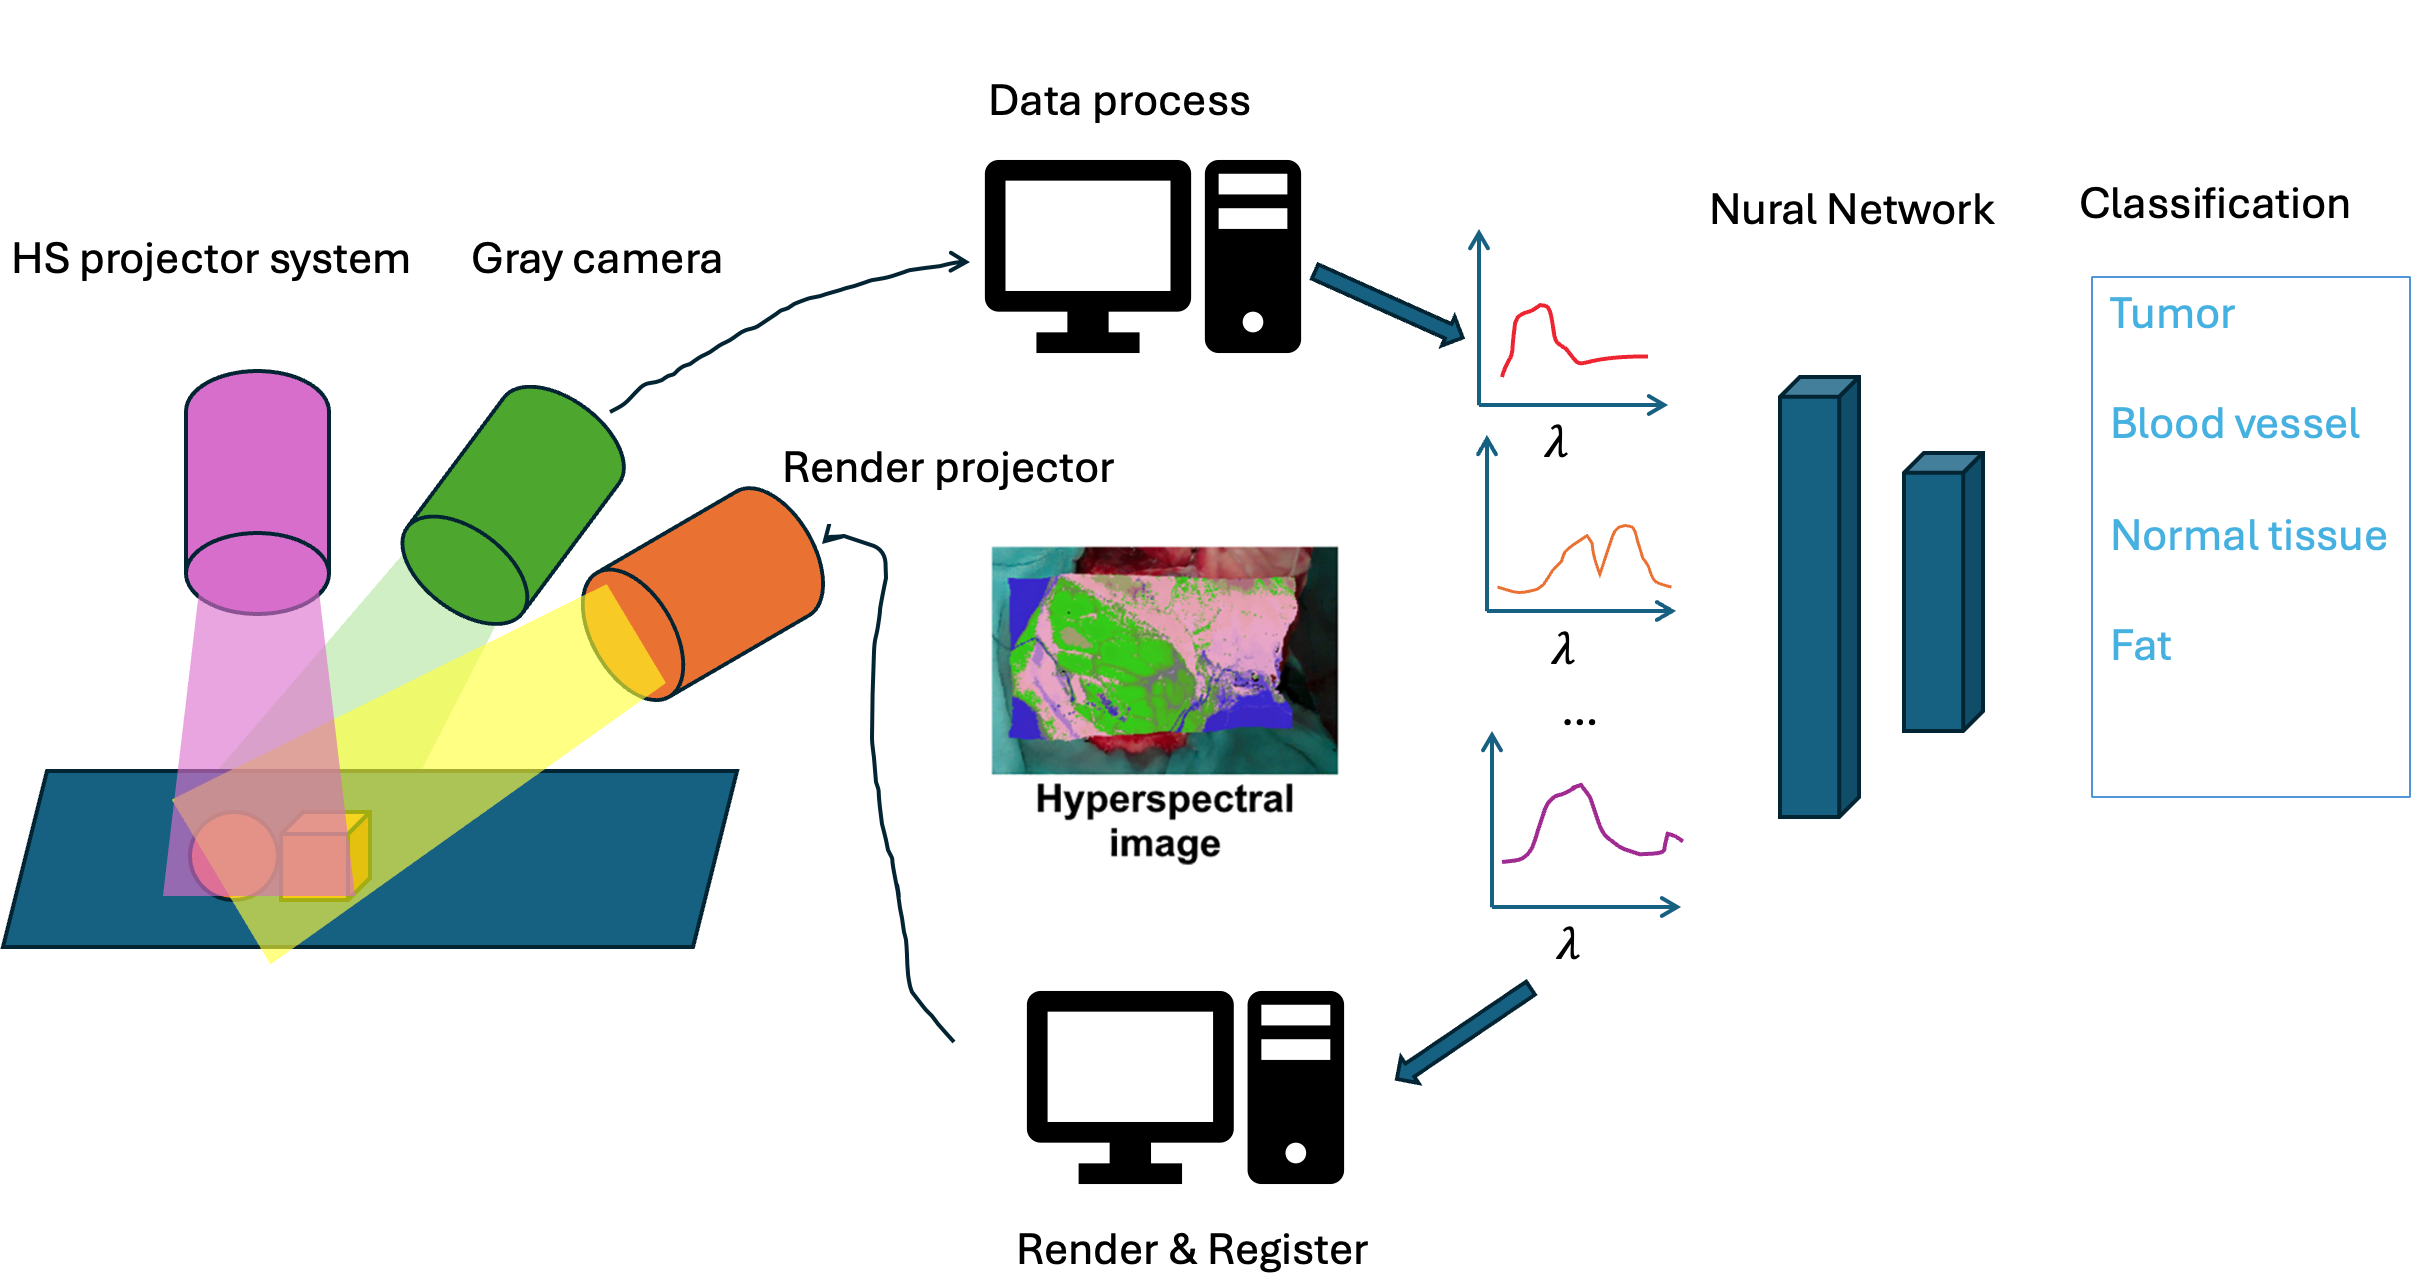
\includegraphics[width=\linewidth]{Figs/system.png}
    \caption{Overall workflow of the proposed real-time SWIR hyperspectral imaging and projection system. A hyperspectral projector illuminates the target scene, a grayscale camera captures the reflected responses, spectral signatures from regions of interest are reconstructed and classified, and the classification results are rendered back onto the object for real-time surgical guidance.}
    \label{fig:system}
\end{figure}


\subsection{Spectral Encoding Strategy}
Fig.~\ref{fig:encodesystem} shows the optical design of the hyperspectral projector (HSP). Light from a halogen lamp is delivered through a gooseneck fiber-optic light guide and focused by a cylindrical lens onto a vertical slit of width 200~\(\mu\)m. The light is collimated by lens L1 and spectrally dispersed along the \(y\)-direction by a transmission diffraction grating (Thorlabs, Visible Transmission Grating, 300 grooves/mm). An achromatic lens L2 focuses the dispersed spectrum onto a digital micromirror device (DMD) (Texas Instruments, DLP6500 0.45 WXGA DMD, \(1920 \times 1080\)). The distances from the grating to L2 and from L2 to the DMD are both equal to the focal length \(f\) of L2, mapping different wavelengths to different DMD positions.

Programmable binary patterns on the DMD perform spectral and spatial modulation. The modulated light is reflected back through L2, recombined by the diffraction grating, and redirected by the beam splitter. A cylindrical lens forms a spectrally encoded stripe at the target plane, while a relay-based magnification lens module adjusts the projection size and a rotating mirror controls the stripe orientation.

\begin{figure}[t]
    \centering
    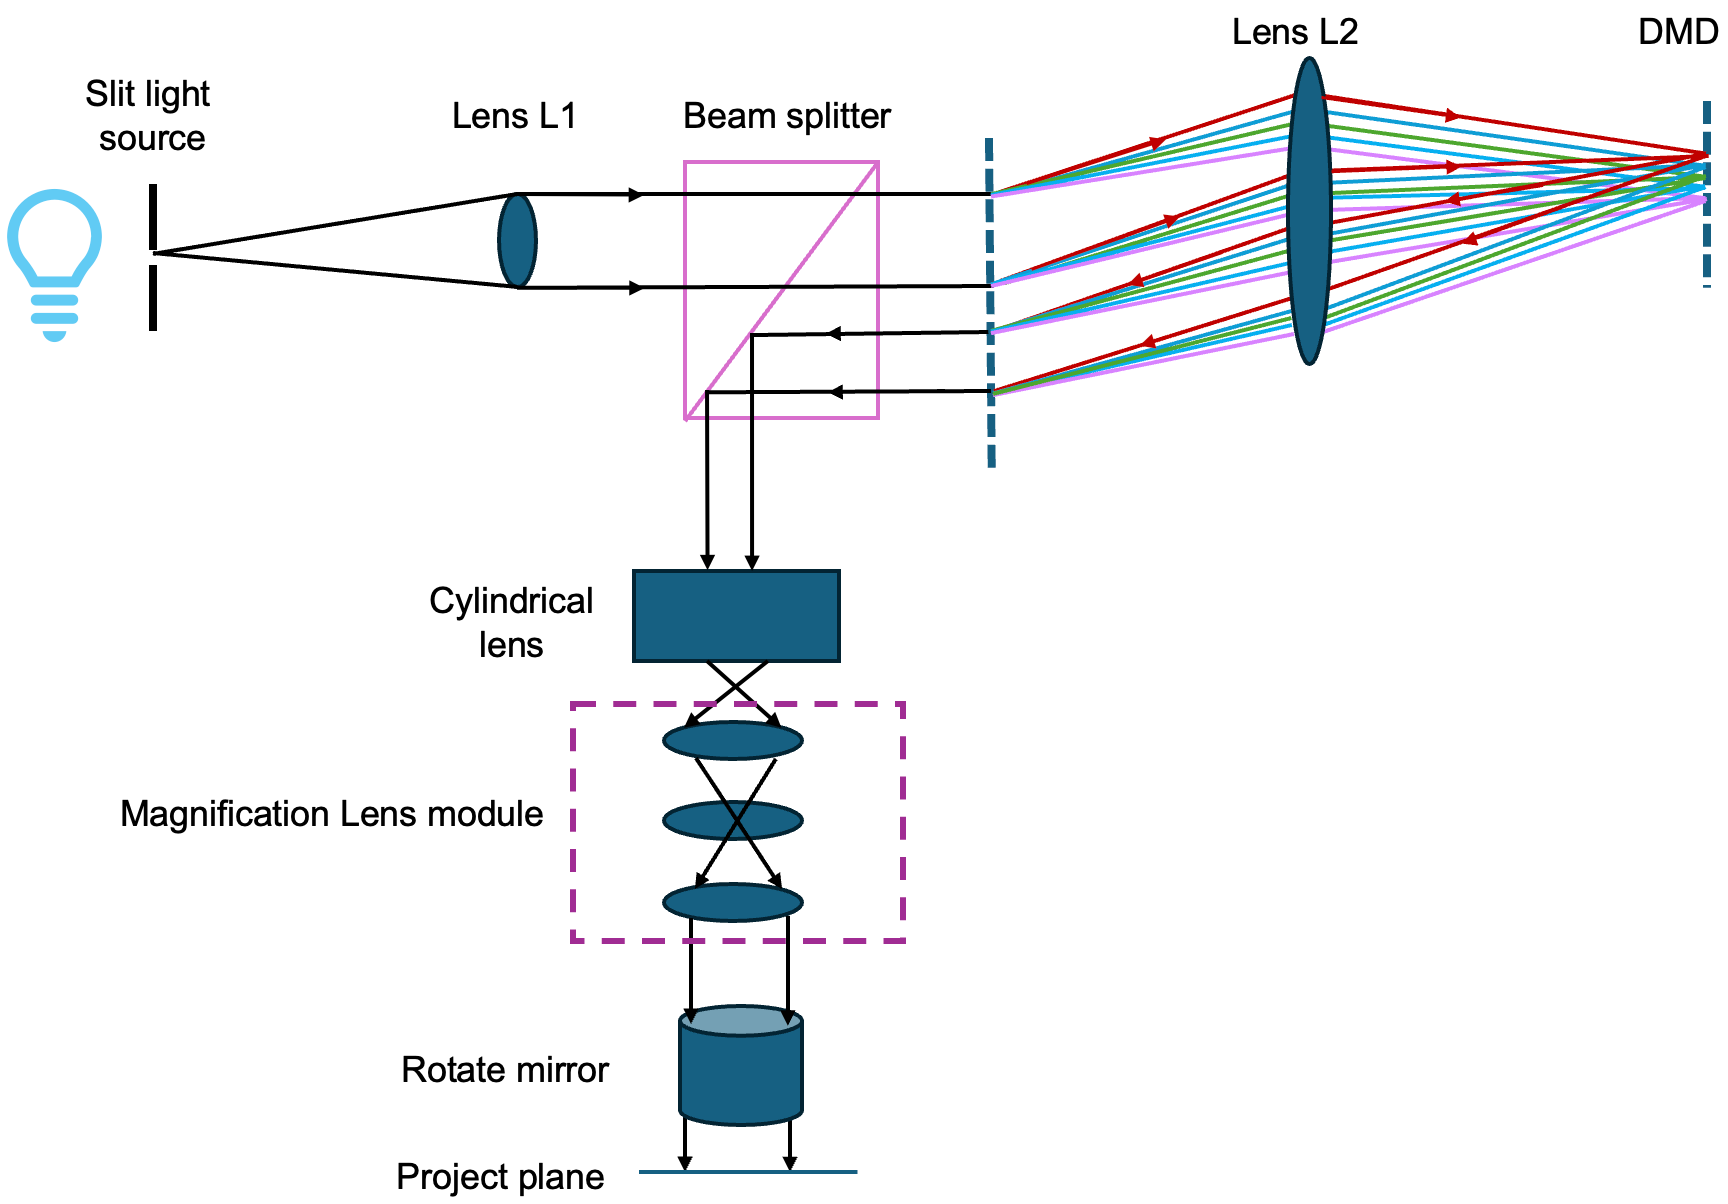
\includegraphics[width=\linewidth]{Figs/encodesystem.png}
    \caption{Optical design of the hyperspectral projector. Broadband light is spectrally dispersed and encoded by the DMD, then recombined and projected as a spectrally modulated stripe. A magnification lens module adjusts the projection size, and a rotating mirror controls the stripe orientation.}
    \label{fig:encodesystem}
\end{figure}



\subsection{Compressive Spectral Reconstruction}
The compressive spectral reconstruction process is illustrated in Fig.~\ref{cs-figure}. Let \(X \in \mathbb{R}^{N \times (h\times w)}\) denote the unknown spectral image, where \(N\) is the number of spectral channels and each column corresponds to the spectrum of one spatial pixel. The measurement matrix is denoted by \(Y \in \mathbb{R}^{N \times (h\times w)}\), where each row represents the response acquired under one projected pattern. The coding matrix \(H \in \mathbb{R}^{N \times N}\) is formed by Hadamard patterns, with each row corresponding to one spectral coding pattern. The forward model can therefore be written as
\[
Y = HX.
\]

Since \(H\) is full-rank, the spectral image \(X\) can be directly recovered by matrix inversion:
\[
X = H^{-1}Y.
\]
In this work, a \(24 \times 24\) Hadamard matrix is used for spectral encoding and reconstruction. For physical implementation, the first Hadamard row, which consists of all ones, is divided into two complementary half-and-half measurements to maintain balanced projection energy. These two measurements are added together during data processing to recover the equivalent all-one pattern response. After this preprocessing step, the full measurement matrix is assembled and used for spectral reconstruction.

\begin{figure}[t]
    \centering
    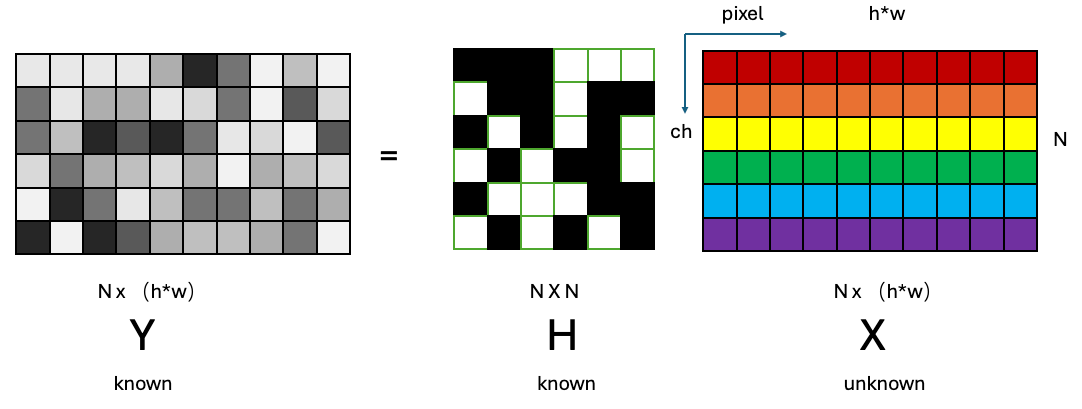
\includegraphics[width=\linewidth]{Figs/cs.png}
    \caption{Compressive spectral reconstruction model based on Hadamard coding, where \(Y=HX\).}
    \label{cs-figure}
\end{figure}

Each element of \(Y\) corresponds to the pixel intensity recorded by the grayscale camera under one Hadamard illumination pattern. Therefore, the measurement matrix \(Y\) is formed by vectorizing the captured image sequence, where each row represents the vectorized image acquired at one spectral coding pattern.

After solving the linear model to obtain \(X\), the reconstructed spectral data are reshaped back to the original spatial dimensions of the captured images. In this representation, each spectral channel corresponds to a reconstructed image of size \(h \times w\). Regions of interest (ROIs) are first selected in the measurement image domain, and the corresponding spatial locations are then used to extract the same regions across all reconstructed spectral channels.

To improve robustness against noise and local intensity variations, a median filter is applied within each ROI for every spectral channel. The filtered intensity values from all channels are then combined to form the final spectral signature associated with the selected material or tissue region.

\section{Results}

\subsection{Spectral Channel Calibration}

\begin{figure}[t]
    \centering
    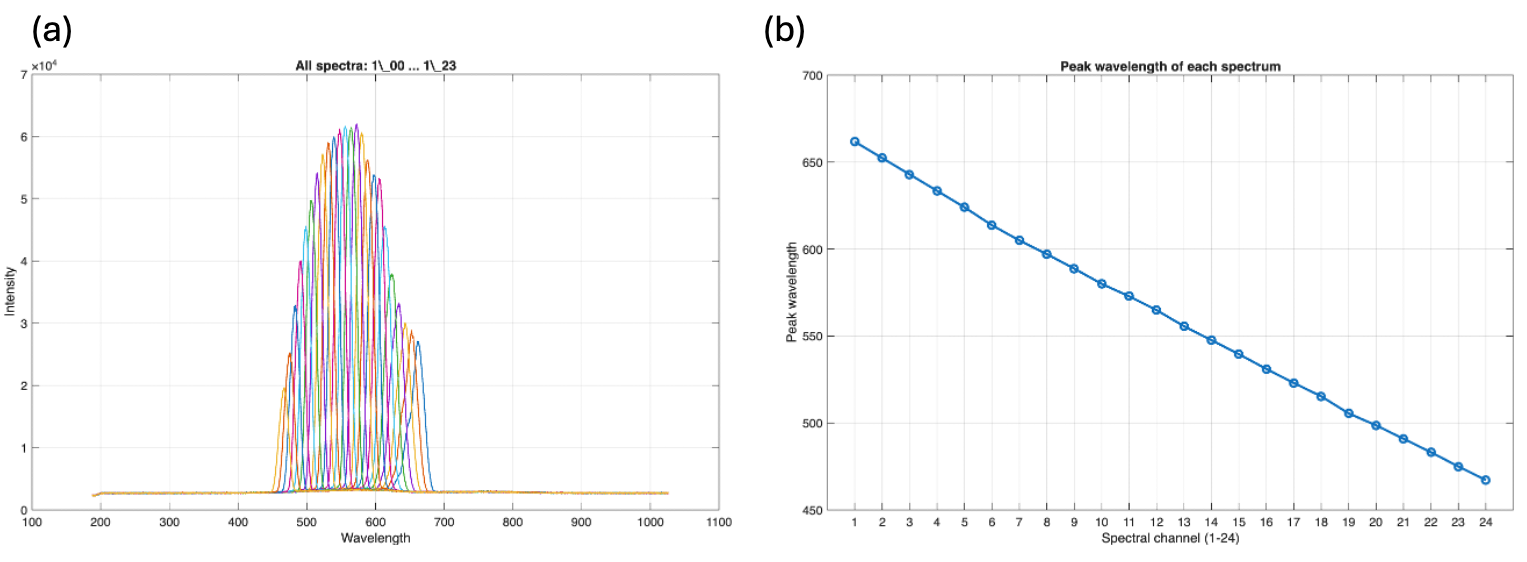
\includegraphics[width=\linewidth]{Figs/spectrum.png}
    \caption{Spectral channel calibration results. (a) Measured spectra of the 24 spectral channels. (b) Peak wavelength of each channel, showing an approximately linear relationship with channel index.}
    \label{spectrum}
\end{figure}

To characterize the spectral encoding performance of the hyperspectral projector, a spectral channel calibration experiment was conducted. The dispersion direction on the DMD was divided into 24 equally spaced regions along the \(y\)-axis. A raster scanning strategy was employed to sequentially project narrow spectral bands corresponding to each region, and the resulting spectra were measured.

Fig.~\ref{spectrum}(a) shows the measured spectra of all 24 channels. The combined result demonstrates that the system provides continuous spectral coverage from 450\,nm to 680\,nm with approximately uniform channel spacing. This confirms that the DMD-based spectral encoding enables controlled selection of wavelength bands.

Fig.~\ref{spectrum}(b) presents the peak wavelength extracted from each measured spectrum as a function of channel index. The peak wavelength exhibits an approximately linear relationship with channel number, indicating that the spectral dispersion mapping onto the DMD is well calibrated. This linear trend verifies the effectiveness and stability of the spectral channel design, providing a reliable basis for subsequent spectral reconstruction and material classification experiments.

\subsection{Spectral Reconstruction}



\begin{figure}[t]
    \centering
    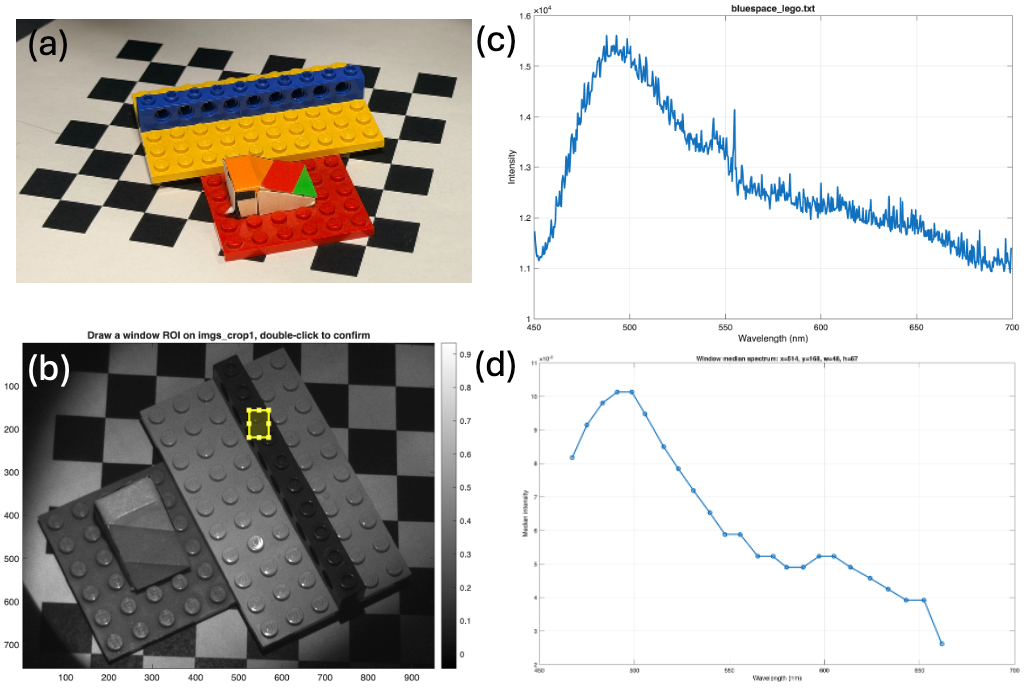
\includegraphics[width=\linewidth]{Figs/reconstructionresult.png}
    \caption{Spectral reconstruction validation. (a) Photograph of the test object composed of Lego bricks with different colors. (b) Grayscale measurement image captured by the camera with the selected ROI marked. (c) Reference spectrum of the blue Lego measured using a spectrometer. (d) Reconstructed spectrum of the blue Lego obtained using the compressive hyperspectral imaging method.}
    \label{fig:spectralreconstruction}
\end{figure}

To validate the spectral reconstruction capability of the proposed compressive hyperspectral imaging system, experiments were conducted on objects composed of Lego bricks with different colors. Fig.~\ref{fig:spectralreconstruction}(a) shows the test scene, while Fig.~\ref{fig:spectralreconstruction}(b) presents the grayscale measurement image captured under structured hyperspectral illumination. Regions of interest (ROIs) were selected from the measurement image for spectral analysis.

The reference spectrum of the blue Lego region measured using a spectrometer is shown in Fig.~\ref{fig:spectralreconstruction}(c). The spectrum reconstructed using the proposed compressive sensing–based hyperspectral imaging method is presented in Fig.~\ref{fig:spectralreconstruction}(d). The reconstructed spectrum exhibits a similar overall shape and peak distribution compared with the reference measurement, demonstrating the effectiveness of the spectral encoding and reconstruction framework.


\section{Discussion}

The results demonstrate that the proposed compressive hyperspectral imaging framework can achieve reliable spectral calibration and reconstruct material spectra with good agreement to spectrometer measurements, validating the effectiveness of spectral multiplexing at the illumination stage. By combining a hyperspectral projector, a grayscale camera, and computational decoding, the system provides a simple and potentially low-cost solution for accelerated hyperspectral imaging and real-time visual feedback. In future work, we will extend this framework to three-dimensional reconstruction and further implement it in the SWIR range, with the goal of achieving simultaneous spectral reconstruction and 3D imaging for surgical applications.

\section{Acknowledgements}

The authors would like to thank the funding from Rice University.
the coding can be find on github https://github.com/matatazzy/ELEC594spr26.git

\section{Credit Author Statement}
Yunan Wang: Investigation, Writing – original draft, Data curation, Software.
Lauren Gold: Conceptualization.
Kevin F. Kelly: Conceptualization, Methodology, Resources, Supervision.
Robert LiKamWa: Conceptualization, Methodology, Resources, Supervision.
% Keep your text and graphic files separate until after the text has been 
% formatted and styled. Do not number text heads---{\LaTeX} will do that 
% for you.

% \subsection{Abbreviations and Acronyms}\label{AA}
% Define abbreviations and acronyms the first time they are used in the text, 
% even after they have been defined in the abstract. Abbreviations such as 
% IEEE, SI, MKS, CGS, ac, dc, and rms do not have to be defined. Do not use 
% abbreviations in the title or heads unless they are unavoidable.

% \subsection{Units}
% \begin{itemize}
% \item Use either SI (MKS) or CGS as primary units. (SI units are encouraged.) English units may be used as secondary units (in parentheses). An exception would be the use of English units as identifiers in trade, such as ``3.5-inch disk drive''.
% \item Avoid combining SI and CGS units, such as current in amperes and magnetic field in oersteds. This often leads to confusion because equations do not balance dimensionally. If you must use mixed units, clearly state the units for each quantity that you use in an equation.
% \item Do not mix complete spellings and abbreviations of units: ``Wb/m\textsuperscript{2}'' or ``webers per square meter'', not ``webers/m\textsuperscript{2}''. Spell out units when they appear in text: ``. . . a few henries'', not ``. . . a few H''.
% \item Use a zero before decimal points: ``0.25'', not ``.25''. Use ``cm\textsuperscript{3}'', not ``cc''.)
% \end{itemize}

% \subsection{Equations}
% Number equations consecutively. To make your 
% equations more compact, you may use the solidus (~/~), the exp function, or 
% appropriate exponents. Italicize Roman symbols for quantities and variables, 
% but not Greek symbols. Use a long dash rather than a hyphen for a minus 
% sign. Punctuate equations with commas or periods when they are part of a 
% sentence, as in:
% \begin{equation}
% a+b=\gamma\label{eq}
% \end{equation}

% Be sure that the 
% symbols in your equation have been defined before or immediately following 
% the equation. Use ``\eqref{eq}'', not ``Eq.~\eqref{eq}'' or ``equation \eqref{eq}'', except at 
% the beginning of a sentence: ``Equation \eqref{eq} is . . .''

% \subsection{\LaTeX-Specific Advice}

% Please use ``soft'' (e.g., \verb|\eqref{Eq}|) cross references instead
% of ``hard'' references (e.g., \verb|(1)|). That will make it possible
% to combine sections, add equations, or change the order of figures or
% citations without having to go through the file line by line.

% Please don't use the \verb|{eqnarray}| equation environment. Use
% \verb|{align}| or \verb|{IEEEeqnarray}| instead. The \verb|{eqnarray}|
% environment leaves unsightly spaces around relation symbols.

% Please note that the \verb|{subequations}| environment in {\LaTeX}
% will increment the main equation counter even when there are no
% equation numbers displayed. If you forget that, you might write an
% article in which the equation numbers skip from (17) to (20), causing
% the copy editors to wonder if you've discovered a new method of
% counting.

% {\BibTeX} does not work by magic. It doesn't get the bibliographic
% data from thin air but from .bib files. If you use {\BibTeX} to produce a
% bibliography you must send the .bib files. 

% {\LaTeX} can't read your mind. If you assign the same label to a
% subsubsection and a table, you might find that Table I has been cross
% referenced as Table IV-B3. 

% {\LaTeX} does not have precognitive abilities. If you put a
% \verb|\label| command before the command that updates the counter it's
% supposed to be using, the label will pick up the last counter to be
% cross referenced instead. In particular, a \verb|\label| command
% should not go before the caption of a figure or a table.

% Do not use \verb|\nonumber| inside the \verb|{array}| environment. It
% will not stop equation numbers inside \verb|{array}| (there won't be
% any anyway) and it might stop a wanted equation number in the
% surrounding equation.

% \subsection{Some Common Mistakes}\label{SCM}
% \begin{itemize}
% \item The word ``data'' is plural, not singular.
% \item The subscript for the permeability of vacuum $\mu_{0}$, and other common scientific constants, is zero with subscript formatting, not a lowercase letter ``o''.
% \item In American English, commas, semicolons, periods, question and exclamation marks are located within quotation marks only when a complete thought or name is cited, such as a title or full quotation. When quotation marks are used, instead of a bold or italic typeface, to highlight a word or phrase, punctuation should appear outside of the quotation marks. A parenthetical phrase or statement at the end of a sentence is punctuated outside of the closing parenthesis (like this). (A parenthetical sentence is punctuated within the parentheses.)
% \item A graph within a graph is an ``inset'', not an ``insert''. The word alternatively is preferred to the word ``alternately'' (unless you really mean something that alternates).
% \item Do not use the word ``essentially'' to mean ``approximately'' or ``effectively''.
% \item In your paper title, if the words ``that uses'' can accurately replace the word ``using'', capitalize the ``u''; if not, keep using lower-cased.
% \item Be aware of the different meanings of the homophones ``affect'' and ``effect'', ``complement'' and ``compliment'', ``discreet'' and ``discrete'', ``principal'' and ``principle''.
% \item Do not confuse ``imply'' and ``infer''.
% \item The prefix ``non'' is not a word; it should be joined to the word it modifies, usually without a hyphen.
% \item There is no period after the ``et'' in the Latin abbreviation ``et al.''.
% \item The abbreviation ``i.e.'' means ``that is'', and the abbreviation ``e.g.'' means ``for example''.
% \end{itemize}
% An excellent style manual for science writers is \cite{b7}.

% \subsection{Authors and Affiliations}
% \textbf{The class file is designed for, but not limited to, six authors.} A 
% minimum of one author is required for all conference articles. Author names 
% should be listed starting from left to right and then moving down to the 
% next line. This is the author sequence that will be used in future citations 
% and by indexing services. Names should not be listed in columns nor group by 
% affiliation. Please keep your affiliations as succinct as possible (for 
% example, do not differentiate among departments of the same organization).

% \subsection{Identify the Headings}
% Headings, or heads, are organizational devices that guide the reader through 
% your paper. There are two types: component heads and text heads.

% Component heads identify the different components of your paper and are not 
% topically subordinate to each other. Examples include Acknowledgments and 
% References and, for these, the correct style to use is ``Heading 5''. Use 
% ``figure caption'' for your Figure captions, and ``table head'' for your 
% table title. Run-in heads, such as ``Abstract'', will require you to apply a 
% style (in this case, italic) in addition to the style provided by the drop 
% down menu to differentiate the head from the text.

% Text heads organize the topics on a relational, hierarchical basis. For 
% example, the paper title is the primary text head because all subsequent 
% material relates and elaborates on this one topic. If there are two or more 
% sub-topics, the next level head (uppercase Roman numerals) should be used 
% and, conversely, if there are not at least two sub-topics, then no subheads 
% should be introduced.

% \subsection{Figures and Tables}
% \paragraph{Positioning Figures and Tables} Place figures and tables at the top and 
% bottom of columns. Avoid placing them in the middle of columns. Large 
% figures and tables may span across both columns. Figure captions should be 
% below the figures; table heads should appear above the tables. Insert 
% figures and tables after they are cited in the text. Use the abbreviation 
% ``Fig.~\ref{fig}'', even at the beginning of a sentence.

% \begin{table}[htbp]
% \caption{Table Type Styles}
% \begin{center}
% \begin{tabular}{|c|c|c|c|}
% \hline
% \textbf{Table}&\multicolumn{3}{|c|}{\textbf{Table Column Head}} \\
% \cline{2-4} 
% \textbf{Head} & \textbf{\textit{Table column subhead}}& \textbf{\textit{Subhead}}& \textbf{\textit{Subhead}} \\
% \hline
% copy& More table copy$^{\mathrm{a}}$& &  \\
% \hline
% \multicolumn{4}{l}{$^{\mathrm{a}}$Sample of a Table footnote.}
% \end{tabular}
% \label{tab1}
% \end{center}
% \end{table}

% \begin{figure}[htbp]
% \centerline{\includegraphics{fig1.png}}
% \caption{Example of a figure caption.}
% \label{fig}
% \end{figure}

% Figure Labels: Use 8 point Times New Roman for Figure labels. Use words 
% rather than symbols or abbreviations when writing Figure axis labels to 
% avoid confusing the reader. As an example, write the quantity 
% ``Magnetization'', or ``Magnetization, M'', not just ``M''. If including 
% units in the label, present them within parentheses. Do not label axes only 
% with units. In the example, write ``Magnetization (A/m)'' or ``Magnetization 
% \{A[m(1)]\}'', not just ``A/m''. Do not label axes with a ratio of 
% quantities and units. For example, write ``Temperature (K)'', not 
% ``Temperature/K''.

% \section*{Acknowledgment}

\newpage
\bibliographystyle{IEEEtran}
\bibliography{ref}



\end{document}
